\section{Introduction}
\label{section:introduction}

Process Historian is a must in modern IoT applications:
such database is used for storing the time-series readings
from various sensors. Process Historian should hold
the following properties: (i) it should be durable to node failures,
(ii) it should be scalable horizontally, (iii) it should guarantee 
fast writes to the disk, (iv) it should have clean design.

In what follows we present MVP for such database that uses 
Cassandara NoSQL database and Python Flask user facing 
web service. The solution is a 24 hours challenge 
and the source codes can be found in~\cite{git}.


In Figure~\ref{fig:arch} we show rather abstract architecture of our deployment.
Thus in the setup we had 4 nodes deployed in the DigitalOcean
cloud: (i) 3 nodes for Cassandra cluster; (ii) MySQL, Nginx,
and single REST API server were deployed on single computing node;
(iii) we had multiple data generators running on local machine.

\begin{figure}[!hbt]\centering
  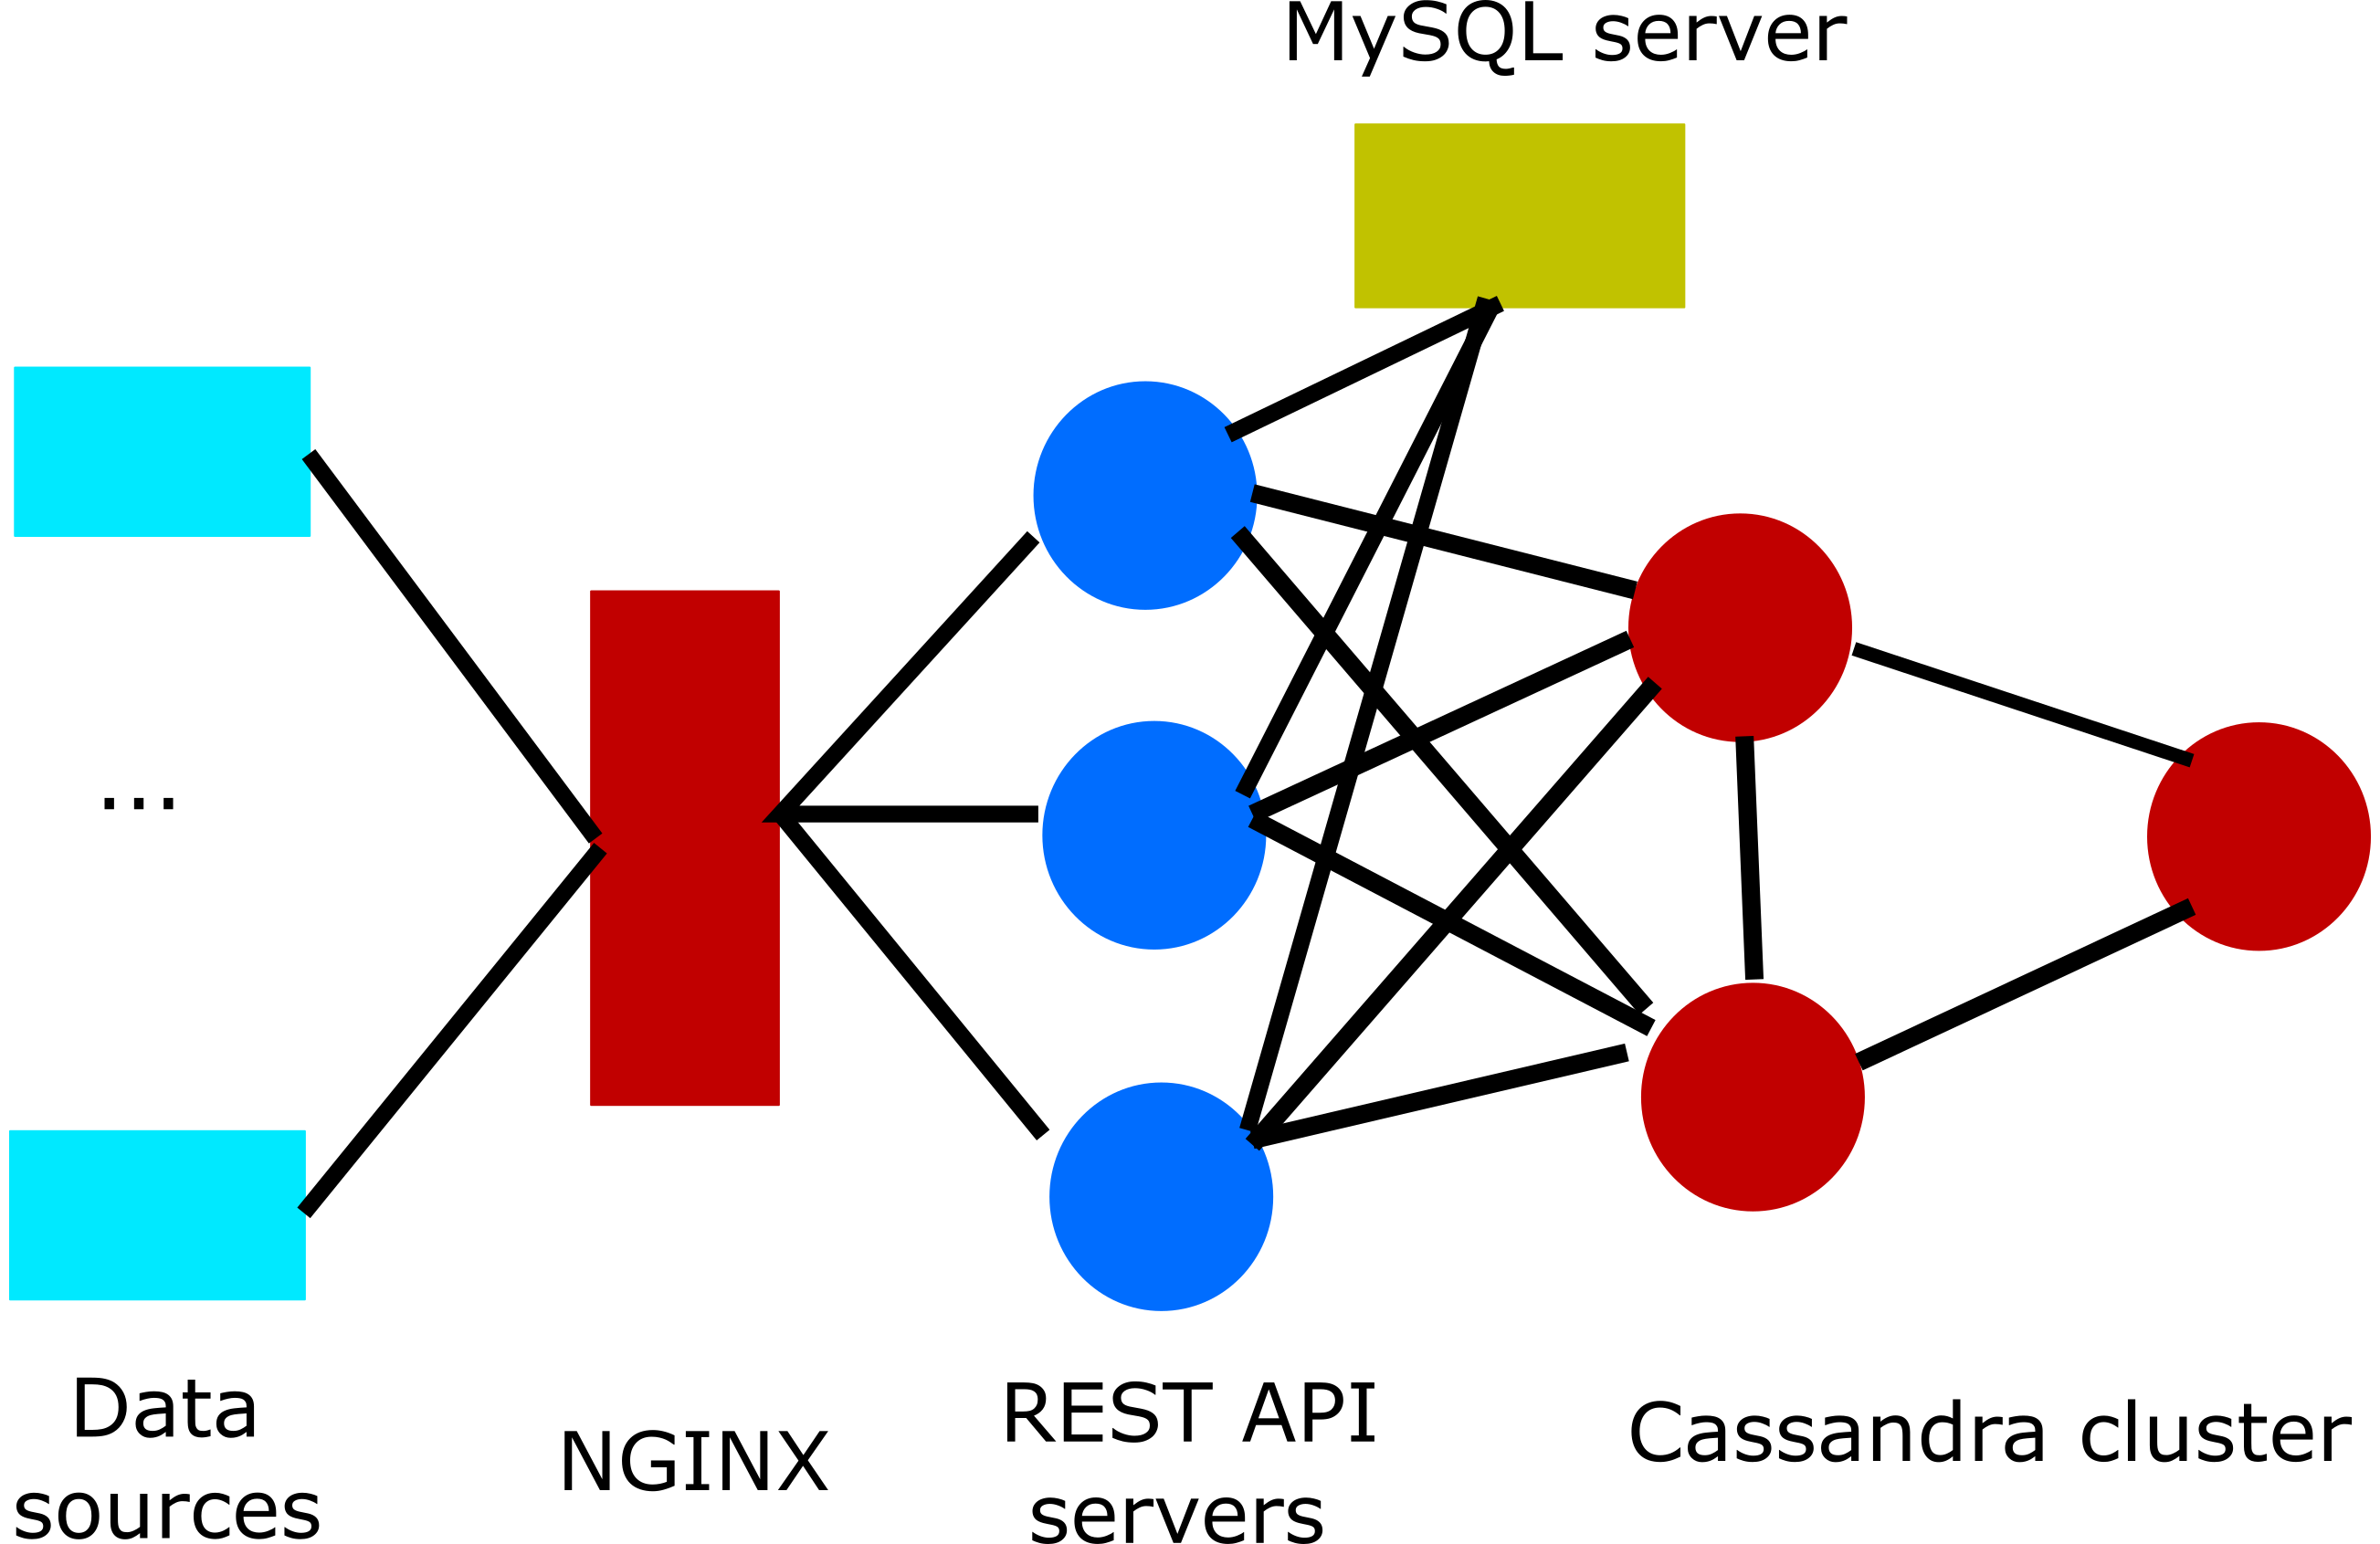
\includegraphics[width=0.45\textwidth]{graphics/arch.png}
  \caption{Process Historian Architecture}
  \label{fig:arch}
\end{figure}

